In this chapter the approach to code testing and a discussion on the problem on how to evaluate the network performance will be presented.


\section{Code testing}
The codebase can be divided in three major components: the sPyNNaker code, the DVS emulator and the network written for the project. 

The sPyNNaker code is already heavily tested. The DVS emulator did not included any unit tests but none were added as part of this project due to time constraints. 

Unit tests had been included in the code written for this project. In particular, all the code that defines the connections between the DVS output and the receptive fields and between the receptive fields and the shapes detectors has unit tests. 

A continuous integration test had been set up using the free tier of \href{http://travis-ci.com}{travis-ci.com} in order to run all the tests at every git push. 


\section{Evaluation of the Network}
Evaluating the performances of this network is quite difficult. In particular, there is no labelled dataset on which the network has been trained. 
The videos used had been generated using a Python script and they cover quite simple scenarios. 

The network performs very well with both squares and diamonds from synthetic videos. The problems with these videos is when the square is moving parallel to the edges of the frame (or the diamond diagonally) as these edges do not generate any spikes, like shown in \cref{fig:square_lr}. 

On synthetic videos the networks is able to recognise quite well shapes of size $5 \times 5$ and $7 \times 7$, as long as their movements on the screen generate enough spikes, for example in the case of a square moving from the top left corner to the bottom right one. 

Another problem is when shapes do not move, hence they do not generate spikes. The eyes do not look at a scene staying still, instead, the eyes move around and these movements are called saccade. A way of simulating saccades for handling still scenes would definitely help to solve this problem. 

Using a webcam as the network input does not produce any meaningful results, as it can be seen in \cref{fig:webcam_results}. The receptive fields, \cref{fig:receptive_fields_webcam_input}, produce spikes in the areas where the shape is moving, but the shape detectors, \cref{fig:shape_webcam_input}, produce too many spikes and a clear location of where the shape is cannot be obtained. 

\begin{figure}[ht]
\centering
\begin{subfigure}{0.45\textwidth}
\centering
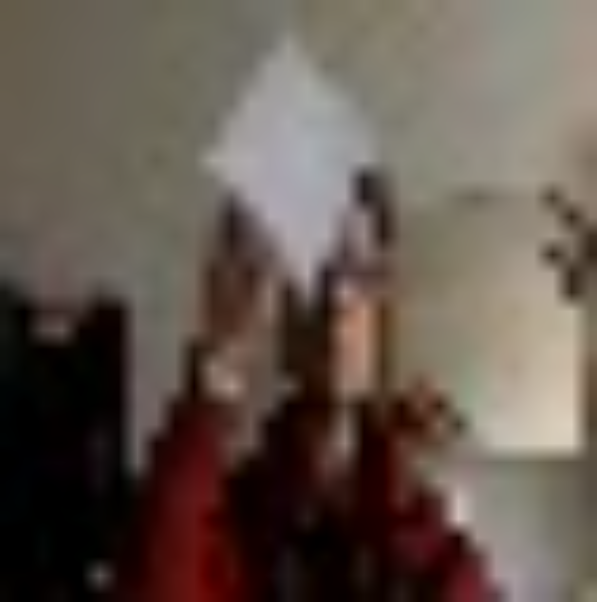
\includegraphics[width=0.5\textwidth]{images/evaluation/webcam_input.png} 
\caption{Screenshot of a recording of a webcam input for tracking the white diamond.}
\label{fig:webcam_input}
\end{subfigure}

\begin{subfigure}{\textwidth}
\centering
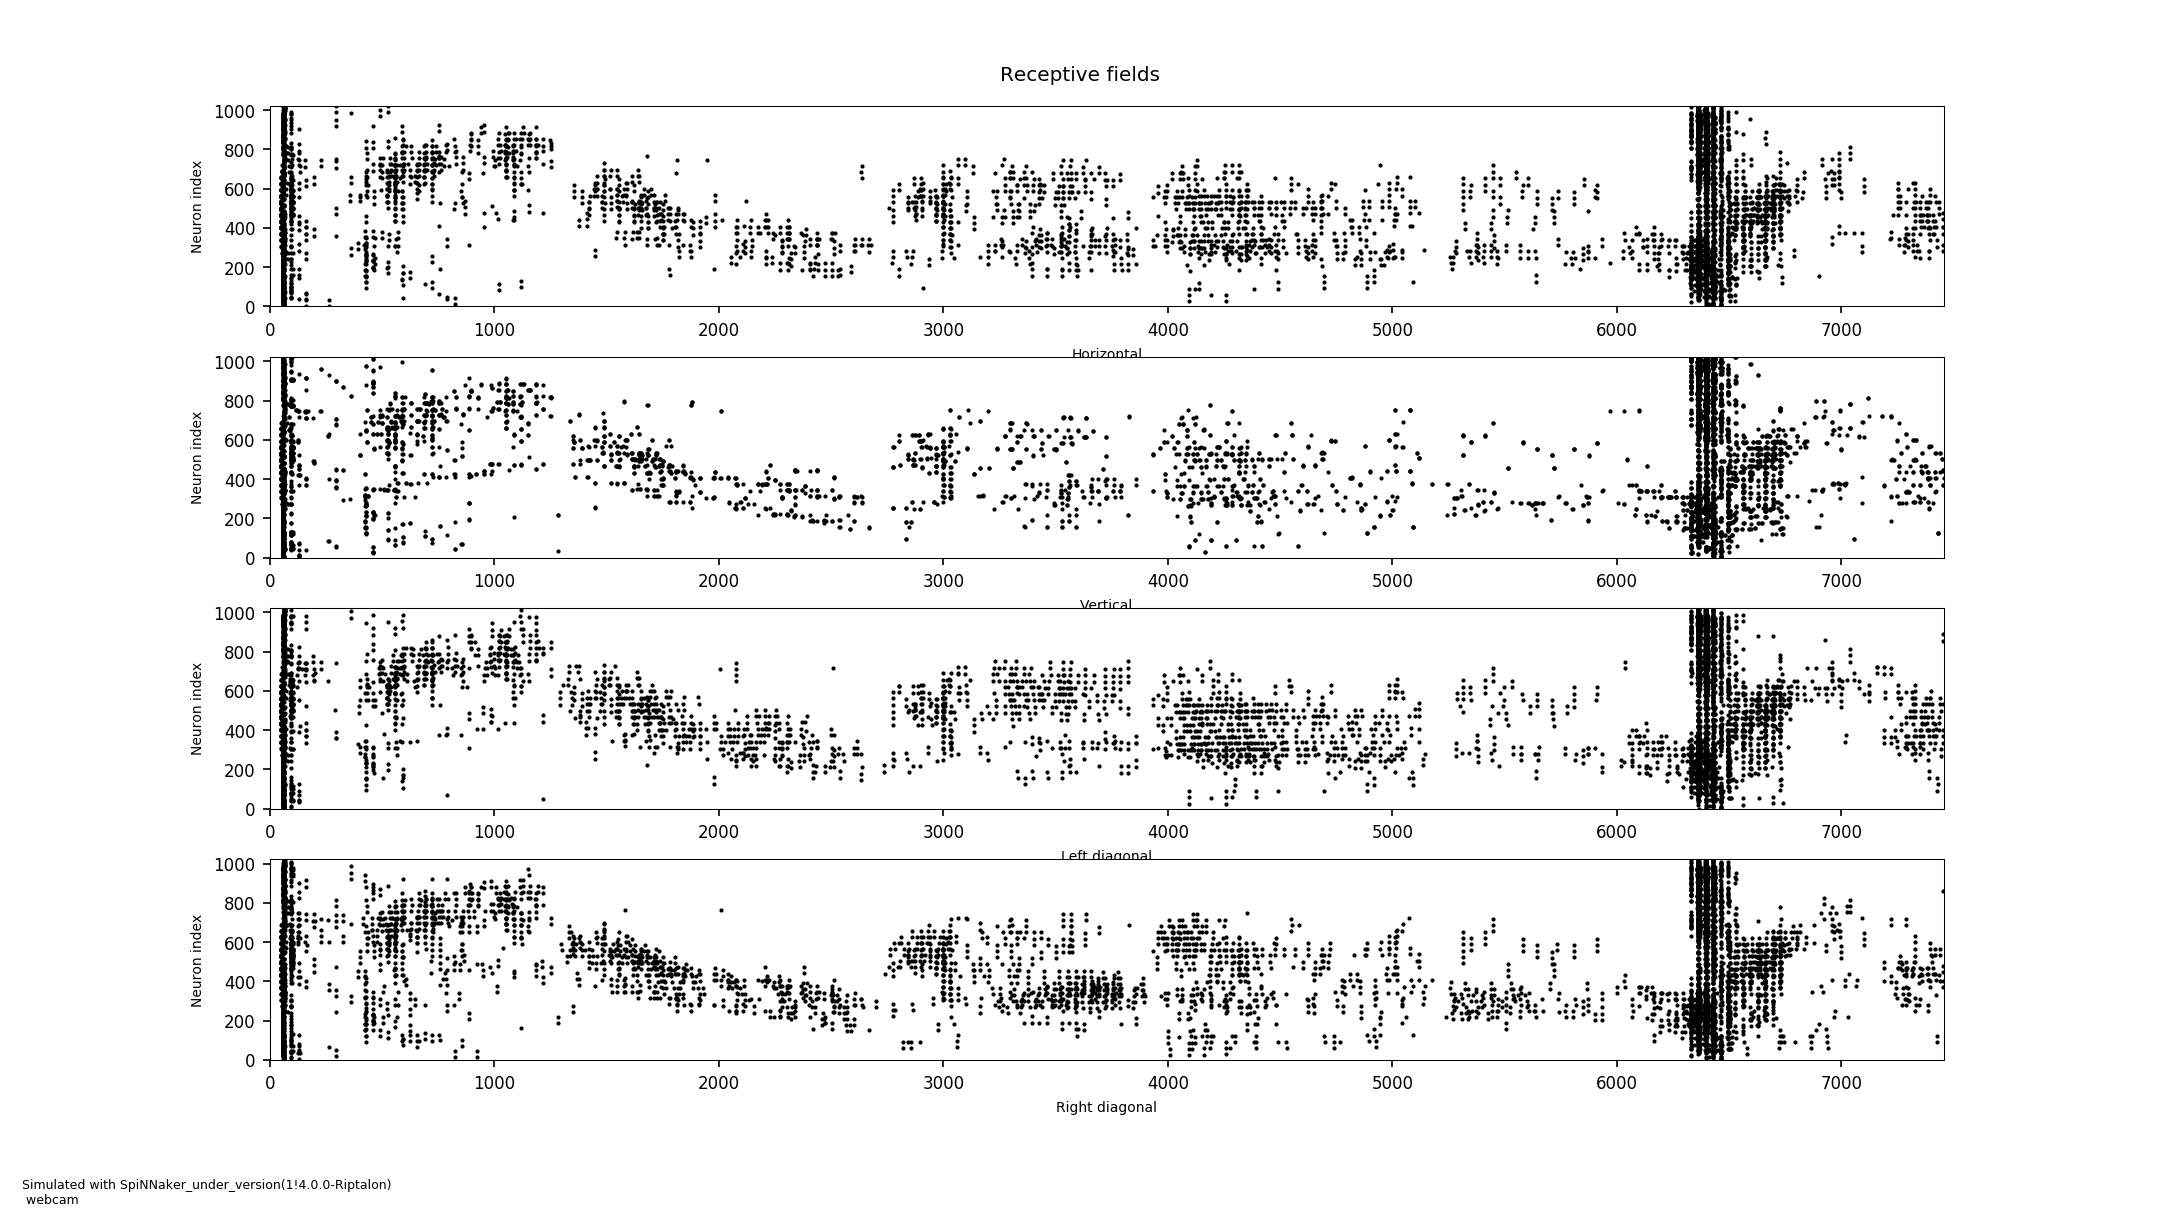
\includegraphics[width=0.75\textwidth]{images/evaluation/receptive_fields_webcam_input.png}
\caption{Receptive fields.}
\label{fig:receptive_fields_webcam_input}
\end{subfigure}

\begin{subfigure}{\textwidth}
\centering
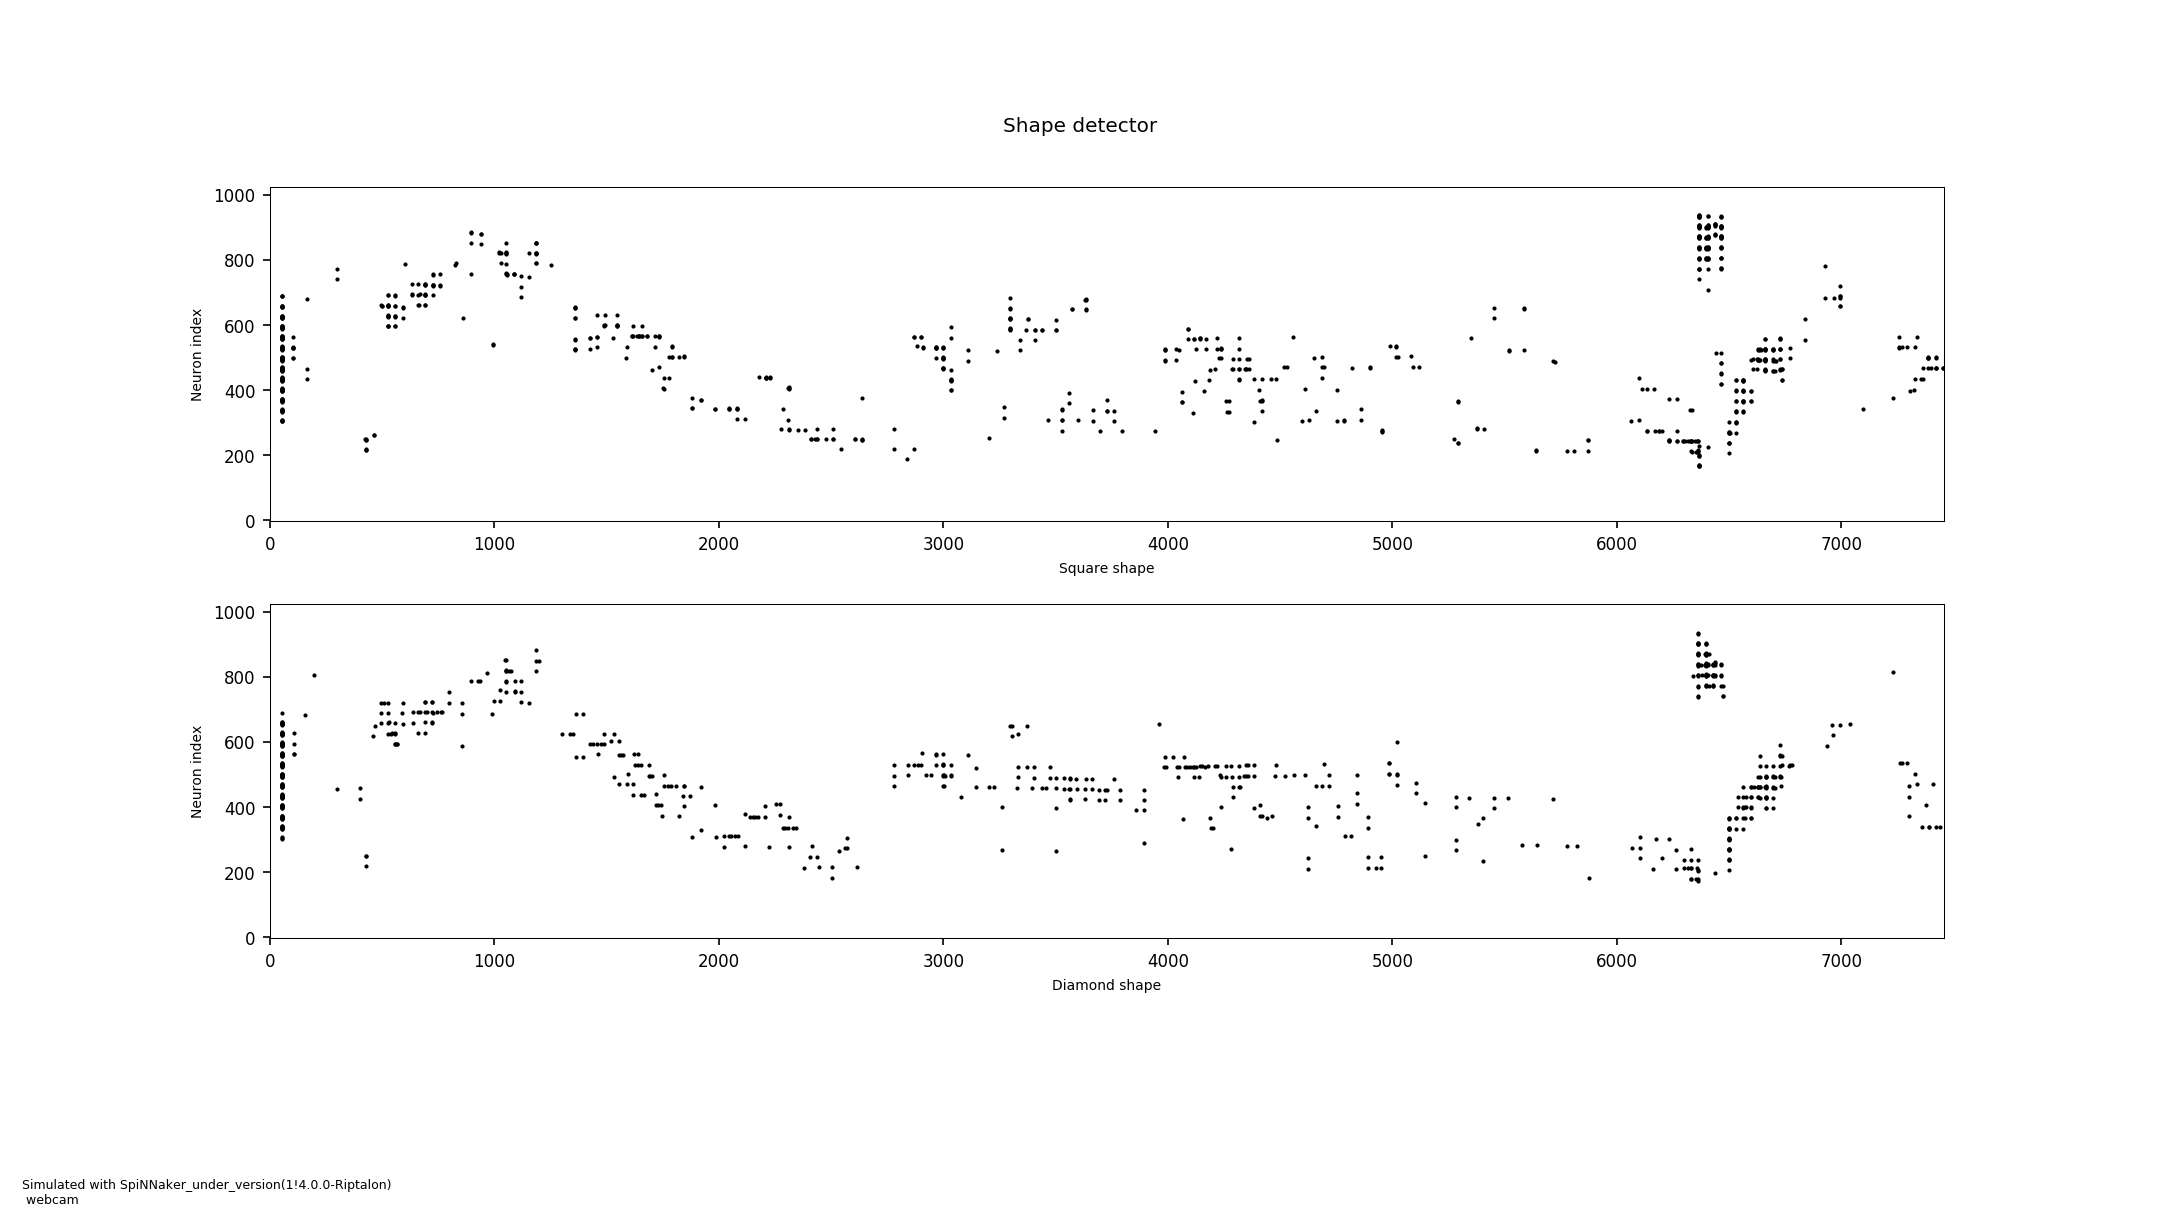
\includegraphics[width=0.75\textwidth]{images/evaluation/shape_webcam_input.png}
\caption{Shape detectors.}
\label{fig:shape_webcam_input}
\end{subfigure}

\caption[Webcam Input Results]{Screenshot and spike trains for the cells populations for a recording of a video registered with a webcam.}
\label{fig:webcam_results}
\end{figure}
